% vim: spelllang=fr

\documentclass[../main.tex]{subfiles}
\graphicspath{{\subfix{../Figures/Chap2/}}}
\begin{document}

\begin{itshape}
Ce deuxième chapitre porte de l'approche directe consistant en l'application d'un algorithme de détection et de suivi des cyclones tropicaux dans les modèles
comme façon de caractériser l'activité cyclonique simulée, ainsi que la façon dont les modèles représentent ces phénomènes. Un cas d'étude est présenté via
l'application du schéma de détection du CNRM à la réanalyse ERA5.
\end{itshape}

\minitoc\newpage
%--------------------------------------

\section{Introduction}\label{sec:intro_chap2}

Les algorithmes de détection et de suivi des HTV dans les modèles consistent à identifier les points de grille qui satisfont des critères thermiques ou
dynamiques associés à un cyclone tropical. Le \cref{chap:chapitre_1}, en particulier la \cref{sec:intro_tracking}, met en évidence la sensibilité de l'activité
cyclonique mesurée au choix de la méthode de détection et montre que ce choix peut aboutir à des conclusions différentes quant au signe du changement dans des
expériences à climat plus chaud. En effet, si tous les traqueurs de TC partagent le même objectif, les méthodologies utilisées dans la littérature présentent
néanmoins une très grande diversité. Les premiers schémas de détection étaient basés uniquement sur la MSLP et la vitesse des vents
\parencite{bengtsson_simulation_1982,broccoli_can_1990}, tandis que \cite{haarsma_tropical_1993,bengtsson_hurricanetype_1995} ajoutèrent à cela des critères sur
la vorticité ainsi qu'un diagnostique sur la présence d'un cœur chaud, dans l'optique de discriminer les perturbations tropicales de leurs homologues
extra-tropicales. \cite{wu_gcm_1992} utilisèrent des critères supplémentaires conçus pour discriminer les perturbations tropicales sèches via un seuil
d'humidité relative, les perturbations équatoriales d'est en interdisant le vent d'est à \hPa{950} au point situé à \ang{4.5} au nord et au sud du cyclone,
ainsi que les perturbations barocliniques en bornant la vitesse du vent d'ouest à \hPa{200} au dessus du centre du cyclone à \ms{5}. Dans
\cite{bengtsson_hurricanetype_1995}, la méthodologie de détection introduit des tests de structure verticale du système, aussi bien sur le profil de vent que de
température. En effet, après avoir identifié un centre cyclonique à travers la vorticité, pression minimum locale et vitesse du vent maximale dans une boîte
autour du système, il s'agit alors de s'assurer de la présence d'une anomalie de température sur l'ensemble de la troposphère, par rapport à la moyenne prise
dans cette boîte, puis de s'assurer également que l'anomalie à la tropopause est supérieure que celle à la couche limite. Un test similaire est réalisé sur le
profil vertical de vent, en imposant que le vent moyen à \hPa{850} supérieur à la moyenne du niveau à \hPa{300}, toujours dans la boîte centrée. Beaucoup
d'algorithmes de détection reprennent cette méthodologie, avec quelques variantes et spécificités. Une grande quantité de méthodologies et de seuils de
détection sont décrits dans \cite{walsh_objectively_2007} ainsi que dans \cite[][Annexe B]{ullrich_tempestextremes_2017}, schémas dans lesquels la définition
d'un TC et les valeurs numériques utilisées pour les divers seuils de détection sont souvent choisis de telle sorte à reproduire au mieux la climatologie
observée \parencite{walsh_objectively_2007,tory_development_2013}.

Parmi les traqueurs possédant des particularités remarquables, le plus communément utilisé est sans aucun doute le schéma de détection TRACK
\parencite{hodges_how_2017}. Ce dernier a la particularité de systématiquement interpoler les champs du modèle à une basse résolution (T63, soit \km{210}),
avant d'appliquer un schéma de détection basé exclusivement sur la vorticité. Cela permettrait de s'affranchir de la sensibilité de la méthode de détection à la
résolution du modèle. Cet algorithme a cependant tendance à détecter une quantité parfois anormalement élevée de systèmes (voir \cref{fig:NTC_HighResMIP_TRACK}
par rapport à la \cref{fig:NTC_HighResMIP}), et est alors particulièrement sujet à la détection de faux-positifs \parencite{bourdin_intercomparison_2022}. La
problématique que TRACK vise à solutionner est néanmoins bien réelle. La résolution du modèle impacte la représentation des TC dans les modèles ce qui implique
que les traqueurs doivent souvent être ajustés pour chaque résolution. Une autre alternative se trouve dans \cite{camargo_improving_2002} où les auteurs ont
proposé une méthode de détection de HTV dont les seuils pour chacune des variables sont déterminées à partir de la climatologie du modèle. Spécifiquement, ces
derniers s'expriment sous la forme $\alpha \sigma + \beta$, où $\alpha$ et $\beta$ sont issues de la climatologie globale du modèle, et où $\sigma$ représente
l'écart type de la variable à l'échelle de chaque bassin océanique. La méthode de \cite{camargo_improving_2002} n'est cependant pas largement répandue,
possiblement parce que d'une part, les valeurs $\alpha$ et $\beta$ pour chacune des variables se déterminent par les densités de probabilités bivariées dont
l'estimation est complexe et laborieuse, et d'autre part parce que cette approche représente un paradigme très différent des traqueurs mentionnés précédemment.
En effet, les traqueurs à seuils fixes visent à appliquer un schéma de fonctionnement conceptuel d'un cyclone tropical au modèle, ce qui permet ensuite
d'établir dans quelle mesure le modèle est capable de simuler des systèmes réalistes, là où la méthode de \cite{camargo_improving_2002} cherche au contraire à
s'affranchir des biais intrinsèques au modèle, en considérant que les TC constituent dans tous les cas les extrêmes des distribution des variables d'intérêt. Il
faut cependant noter que si les traqueurs à seuils absolus permettent d'évaluer des biais de représentation des TC, ils ont également le défaut de rendre
indiscernables les erreurs issues du modèle de celles issues du schéma de détection lui-même, contribuant aux incertitudes quant à l'évolution future de la
fréquence des cyclones tropicaux dans un climat plus chaud mentionnées dans le \cref{chap:chapitre_1}, \cref{sec:intro_tracking}. Ces deux catégories de
traqueurs ont donc chacun leurs avantages et leurs inconvénients.

Ainsi, pour espérer comprendre la divergence entre les projections issues de l'approche directe et indirecte, il est nécessaire de pouvoir évaluer
quantitativement la performance d'un schéma de détection et de suivi objectif de cyclones tropicaux. Une solution consiste à appliquer un schéma de détection à
une simulation dont les trajectoires sont à priori connues d'avance, en utilisant une réanalyse atmosphérique. Les réanalyses combinent des prévisions
météorologiques à court terme avec des observations passées via un modèle et un schéma d'assimilation de données ---~permettant de corriger la trajectoire du
modèle lorsque ce dernier s'éloigne de l'état connu de l'atmosphère~--- invariants sur toute la période d'analyse. Une réanalyse offre donc une vision globale
de l'atmosphère qui est cohérente dans le temps et l'espace et qui intègre au mieux l'ensemble des observations qui y sont intégrées, si bien que le produit
final constitue une excellente estimation de l'état passé de l'atmosphère sur toute la période considérée. Il en résulte que la plupart ---~sinon
l'intégralité~--- des cyclones tropicaux observés et référencés dans la base données IBTrACS, introduite dans le \cref{chap:chapitre_1},
\cref{sec:observations}, sont à priori présents dans une réanalyse.

Dans ce chapitre, on considère le schéma de détection du CNRM, à l'origine conçu pour suivre les dépressions de moyennes latitudes par
\cite{ayrault_nouvelle_2000} puis adapté aux cyclones tropicaux dans \cite{chauvin_response_2006}, et utilisé à cette fin par
\cite{daloz_impact_2012,chauvin_atlantic_2017,chauvin_future_2020,cattiaux_projected_2020}. Des descriptions détaillées du fonctionnement de cet algorithme sont
disponibles dans \cite{chauvin_response_2006}, ainsi que dans la \cref{sec:papier_data_methods}. Spécifiquement, le traqueur du CNRM est appliqué à la réanalyse
ERA5 \parencite{hersbach_era5_2020}. En effet, ERA5 est la dernière en date du CEPMMT et est la première réanalyse mondiale à atteindre une résolution
horizontale de \km{31}, ici interpolée sur une grille à \ang{0.25}. Elle assimile des données issues de plus d'une vingtaine de satellites d'observations
météorologiques, totalisant \num{54} instruments. Aux données satellitaires s'ajoutent les observations \textit{in-situ} composées de stations au sol, bouées
instrumentées, navires marins, radiosondages, radars et avions de reconnaissance. De par sa résolution inédite et la grande diversité des sources observations
qui y sont assimilées, ERA5 constitue donc le choix idéal pour évaluer la capacité du traqueur à détecter les HTV. Dans la \cref{sec:eval_tracker_ERA5}, les
performances du traqueur du CNRM ainsi que sa sensibilité à ses divers seuils de détection sont évaluées sur ERA5, en termes de probabilité de détection
(\textit{Probability of Detection}, POD) et de taux de fausses alarmes (\textit{False Alarm Rate}, FAR). La capacité d'ERA5 à représenter les TC est également
évaluée, via une analyse de leurs caractéristiques en termes d'intensité, de cycle de vie et également via l'étude de leur profiles verticaux. Ces travaux sont
présentés par la publication scientifique dont ils ont fait l'objet \parencite{dulac_assessing_2023}. Un article complémentaire compare les tracks issues de
quatre schémas de détection appliqués à ERA5, dont celui du CNRM \parencite{bourdin_intercomparison_2022}. Enfin, la \cref{sec:complements_papier} présente des
considérations sur le filtrage de systèmes de moyennes latitudes ---~source de biais important dans les schémas de détection de TC---~ ainsi qu'une possible
alternative au FAR et au POD comme métrique d'optimisation, via l'évaluation de la similarité des trajectoires détectées dans ERA5 par rapport aux trajectoires
historiques.

\section{Évaluation du traqueur CNRM sur ERA5 par rapport à IBTrACS}\label{sec:eval_tracker_ERA5}

\subsection{Résumé de l'article}

La réanalyse ERA5 du Centre européen pour les prévisions météorologiques à moyen terme est la première réanalyse mondiale à atteindre une résolution horizontale
de \km{31} et offre donc une occasion unique d'étudier les cyclones tropicaux, et en particulier les champs 3D associés aux TC historiques. A cette fin, un
algorithme de détection et de suivi des TC spécialement calibré pour ce jeu de données est appliqué sur ERA5 ainsi qu'un algorithme d'appariement des
trajectoires conçu pour associer les trajectoires détectées avec celles issues de la base de données IBTrACS dans le but d'évaluer la capacité de la réanalyse à
représenter les cyclones tropicaux Après optimisation du schéma de suivi et l'application d'une technique de filtrage dynamique des systèmes de moyennes
latitudes, il est montré que la majorité des TC d'IBTrACS sont détectés dans ERA5 et que le nombre de fausses alarmes reste raisonnablement bas dans la plupart
des régions. En comparant les trajectoires détectées dans ERA5 avec leurs équivalents IBTrACS, on constate que l'intensité des TC est encore fortement
sous-estimée dans la réanalyse, mais que la distribution de la pression minimale au niveau de la mer est mieux représentée que la vitesse maximale du vent. Par
ailleurs, la comparaison entre les cycles de vie des deux jeux de données met en évidence des différences essentielles entre ERA5 et les best tracks, avec en
particulier un retard avec lequel les TC d'ERA5 atteignent leur pic d'intensité par rapport à IBTrACS, délai qui augmente de manière significative pour les
cyclones les plus forts. Enfin, les structures verticales des TC dans la réanalyse sont analysées et révèlent une intensification nette jusqu'à la catégorie 3
sur l'échelle de Saffir-Simpson, au delà de quoi les différences sont peu discernables.

La version publiée de \cite{dulac_assessing_2023} est présentée dans la \cref{sec:papier} ci-après, avec la permission de l'éditeur \textit{Springer Nature}.

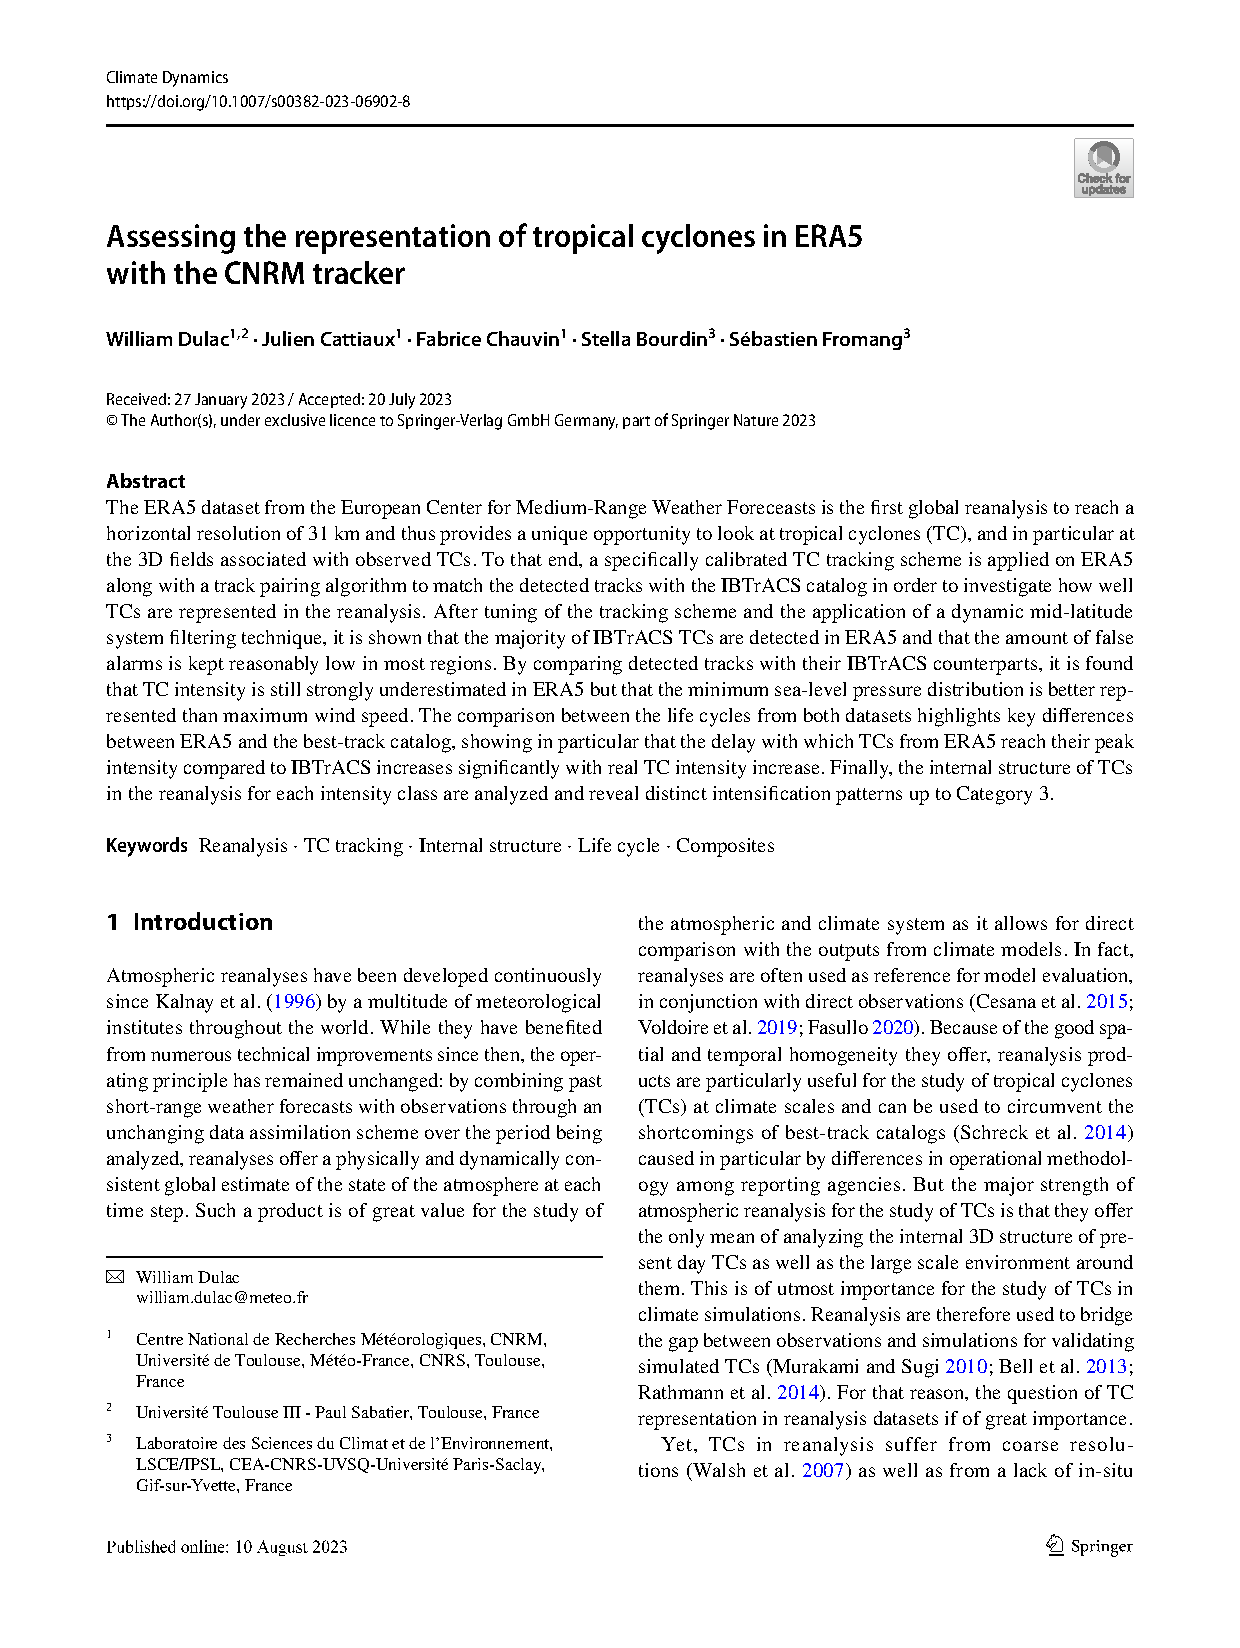
\includepdf[pages=-,pagecommand={\thispagestyle{plain}},offset=5mm 0mm,scale=1,addtotoc=
    {1,subsection,1,Article Climate Dynamics,sec:papier,
     1,subsubsection,2,Introduction,sec:papier_intro,
     2,subsubsection,2,Données et Méthodes,sec:papier_data_methods,
     4,subsubsection,2,Résultats,sec:papier_results,
     10,subsubsection,2,Discussion et conclusion,sec:papier:discussion,
     12,subsubsection,2,Annexe A: Optimisation du traqueur pour ERA5,sec:papier_appendix_A}]{\subfix{../include/dulac2023.pdf}}
%
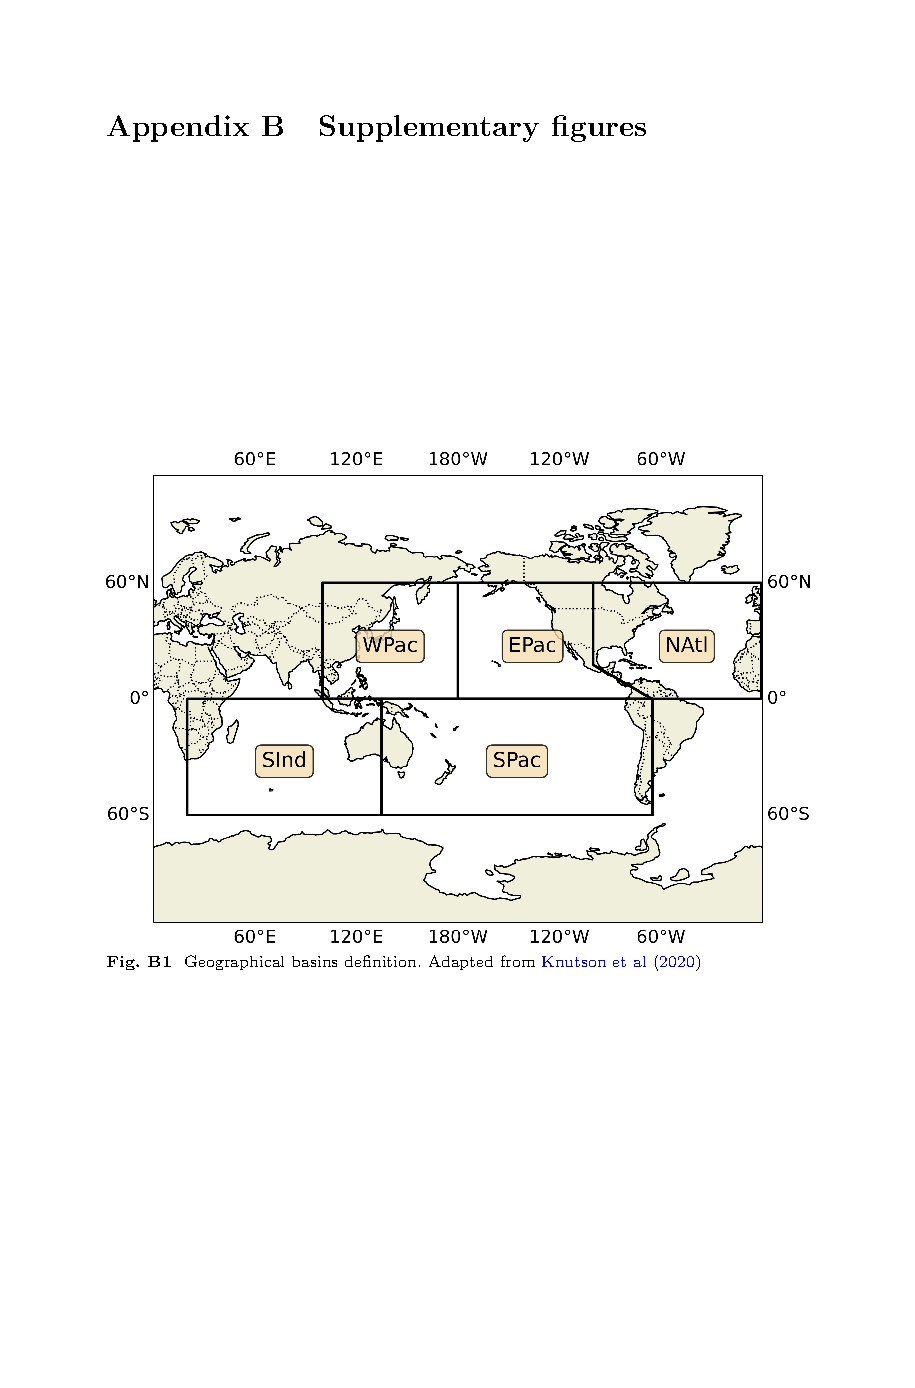
\includepdf[pages=-,pagecommand={\thispagestyle{plain}},offset=5mm 0mm,addtotoc=
{1,subsubsection,2,Annexe B: Figures supplémentaires,sec:papier_appendix_B}]{\subfix{../include/appendix_B_empty.pdf}}

\section{Compléments}\label{sec:complements_papier}

\subsection{Filtrage des systèmes de moyennes latitudes}\label{sec:filtrage_mid_latitudes}

\subsection{Métriques d'évaluation de la similarité des trajectoires}\label{sec:similarité}



%--------------------------------------
\section{Synthèse}

\end{document}
